%!TEX program = xelatex

\documentclass[compress]{beamer}
%--------------------------------------------------------------------------
% Common packages
%--------------------------------------------------------------------------
\usepackage[english]{babel}
\usepackage{pgfpages} % required for notes on second screen
\usepackage{graphicx}
\usepackage{subfigure}
\usepackage{multicol}
\usepackage{color}

\usepackage{tabularx,ragged2e}
\usepackage{booktabs}

\usepackage{setspace}

%--------------------------------------------------------------------------
% Load theme
%--------------------------------------------------------------------------
\usetheme{hri}

\usepackage{dtklogos} % must be loaded after theme
\usepackage{tikz}
\usetikzlibrary{calc,mindmap,backgrounds,positioning,svg.path}



\graphicspath{{figs/}}

\renewcommand{\bf}{\Medium}

\newcommand\given[1][]{\:#1\vert\:}

%--------------------------------------------------------------------------
% General presentation settings
%--------------------------------------------------------------------------
\title{Mutual Modelling in Educational Child-Robot Interaction}
\subtitle{\textit{Does a second level of modelling\\enable higher quality interactions?}}
\date{EDRS candidacy exam}
\author{Alexis D. Jacq}
\institute{Computer-Human Interaction\\for Learning and Instruction {\Medium
EPFL}\\
\& Instituto Sup\'erior T\'ecnico\\  {\Medium
University of Lisbon}}

%--------------------------------------------------------------------------
% Notes settings
%--------------------------------------------------------------------------
%\setbeameroption{show notes on second screen}
%\setbeameroption{hide notes}

\begin{document}

\maketitle

%%%%%%%%%%%%%%%%%%%%%%%%%%%%%%%%%%%%%%%%%%%%%%%%%%%%%%%%%%%%%%%%%%%%%%%%%%%%%%%
%%%%%%%%%%%%%%%%%%%%%%%%%%%%%%%%%%%%%%%%%%%%%%%%%%%%%%%%%%%%%%%%%%%%%%%%%%%%%%%
%%%%%%%%%%%%%%%%%%%%%%%%%%%%%%%%%%%%%%%%%%%%%%%%%%%%%%%%%%%%%%%%%%%%%%%%%%%%%%%

\section{Introduction}
\begin{frame}{Mutual modelling in HRI}
    \begin{figure}
        \centering
        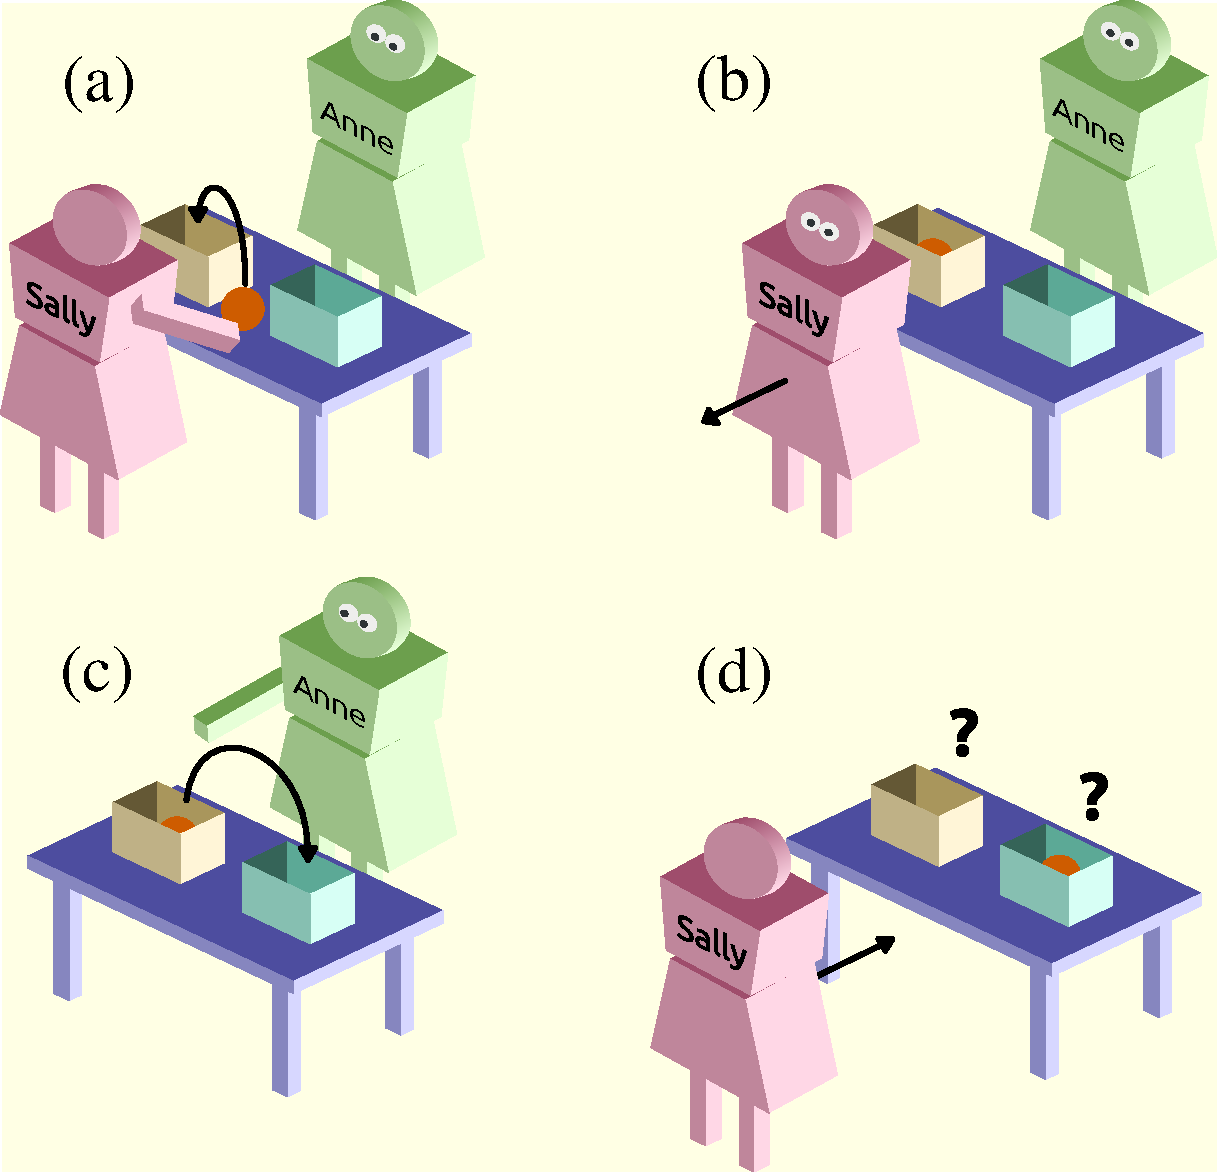
\includegraphics[width=0.7\columnwidth]{sally_ann}
    \end{figure}
\end{frame}

\begin{frame}{The CoWriter activity}
	\begin{figure}
        \centering
        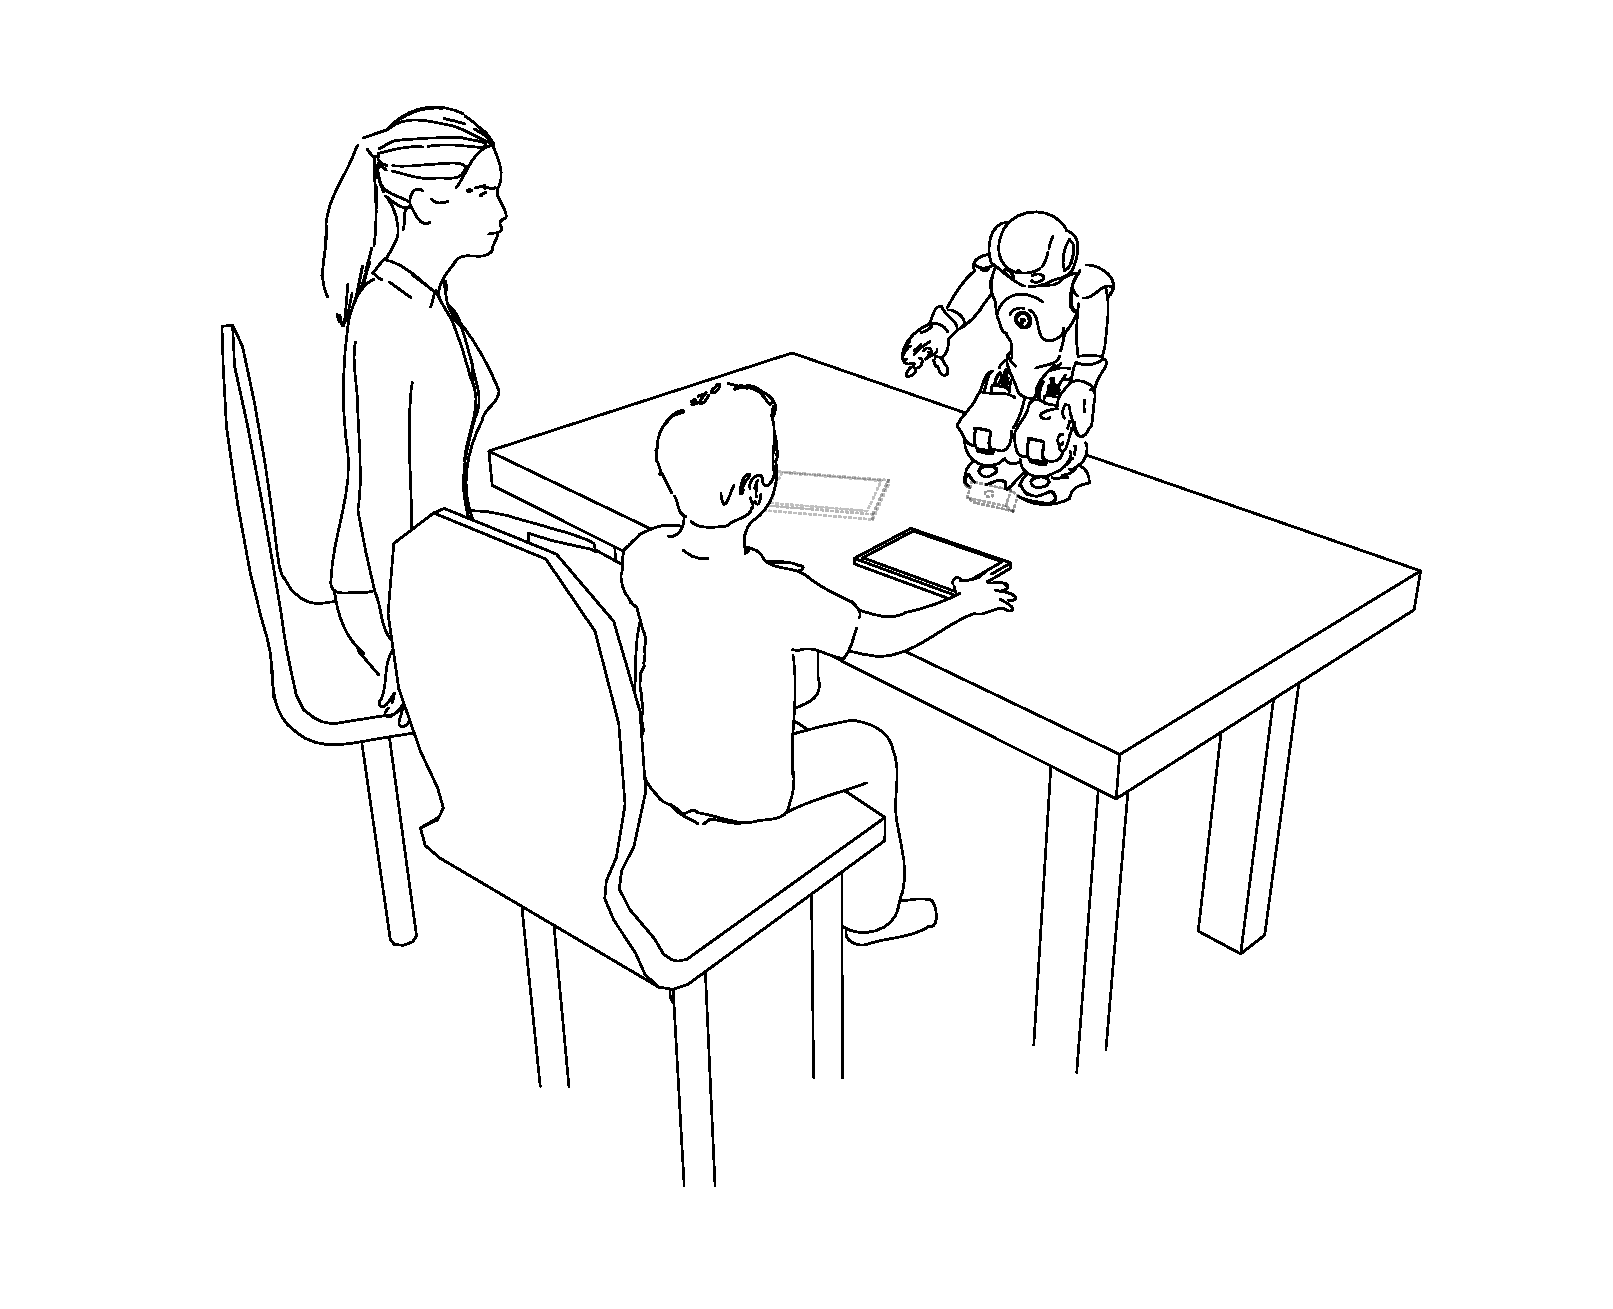
\includegraphics[width=0.8\columnwidth]{experimental_setup}
    \end{figure}
\end{frame}


%%%%%%%%%%%%%%%%%%%%%%%%%%%%%%%%%%%%%%%%%%%%%%%%%%%%%%%%%%%%%%%%%%%%%%%%%%%%%%%%%
\section{Framework}

\begin{frame}{Definitions}
\begin{itemize}
	\item 1st-order agents
	\item 2nd-order agents
	\item nth-order agents
\end{itemize}
\end{frame}

\begin{frame}{Definitions}
\begin{itemize}
	\item perceived variables
	\item abstract variables
	\item model of an agent
\end{itemize}
\end{frame}

\begin{frame}{Notations}
\begin{itemize}
	\item $\textbf{M}_{\textbf{A}}$
	\item $\textbf{M}_{\textbf{A,B}}$
	\item $\textbf{M}_{\textbf{A,B,C,D}}$
	\item $$\displaystyle \textbf{M}^t_{\textbf{A}}(X) = x^t$$
\end{itemize}
\end{frame}


\begin{frame}{Expected causalities}
$$ \mathbb{P}\left[\textit{mental state}\,\given[\Big]\,\textit{behaviour}\right]$$
$$ \mathbb{P}\left[\textit{abstract variables}\,\given[\Big]\,\textit{perveived variables}\right]$$
\end{frame}

\begin{frame}{Expected causalities}
$$ \mathbb{P}\left[\textbf{M}^t_{\textbf{C,R}}(X)\,\given[\Big]\,\textbf{M}^t_{\textbf{C,R}}(Y)>0\right]\sim 1$$
$$\mathbb{P}\left[ \textbf{M}^{t_0}_{\textbf{C}}(X) \given[\Big] \textbf{M}^{t_0}_{\textbf{C}}(Y)=\textit{``robot's hand"} \bigcap\limits^{t_0+\theta}_{t_1>t_0} \textbf{M}^{t_1}_{\textbf{C}}(Y)\neq\textit{``target object"}\right]\sim 0$$
\end{frame}


%%%%%%%%%%%%%%%%%%%%%%%%%%%%%%%%%%%%%%%%%%%%%%%%%%%%%%%%%%%%%%%%%%%%%%%%%%%%%%%%
\section{Cognitive architecture}

\begin{frame}{Global description}
	\begin{figure}
        \centering
        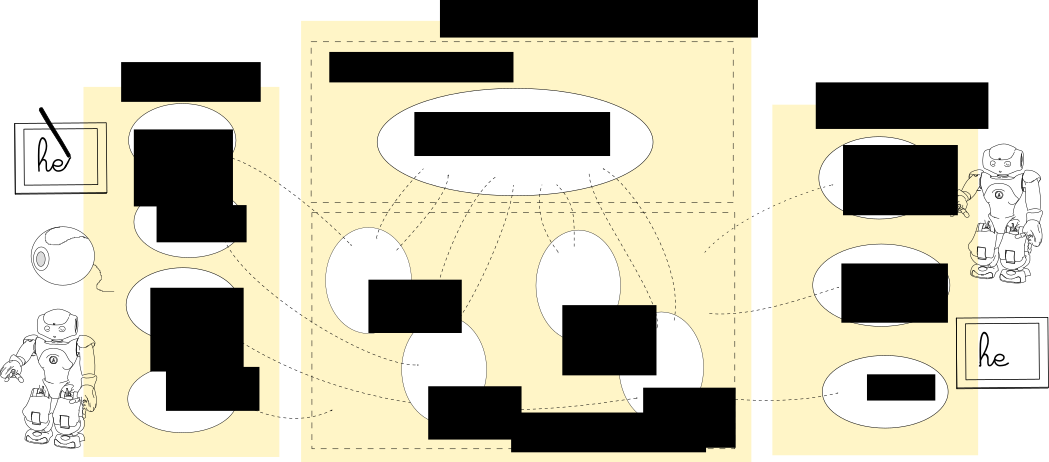
\includegraphics[width=1\columnwidth]{cognitive_archi}
    \end{figure}
\end{frame}

\begin{frame}{Decision making}
\begin{enumerate}
\item \textcolor{blue}{Wizard-of-Oz}: A human takes decisions; the robot learns
\item \textcolor{blue}{Mixed-initiative}: The robot makes suggestions; a human agrees or disagrees
\item \textcolor{blue}{Autonomous}: The robot makes decisions
\end{enumerate}
\end{frame}

%%%%%%%%%%%%%%%%%%%%%%%%%%%%%%%%%%%%%%%%%%%%%%%%%%%%%%%%%%%%%%%%%%%%%%%%%%%%%%%%
\section{Implementation}

\begin{frame}{ROS nodes}
	\begin{figure}
        \centering
        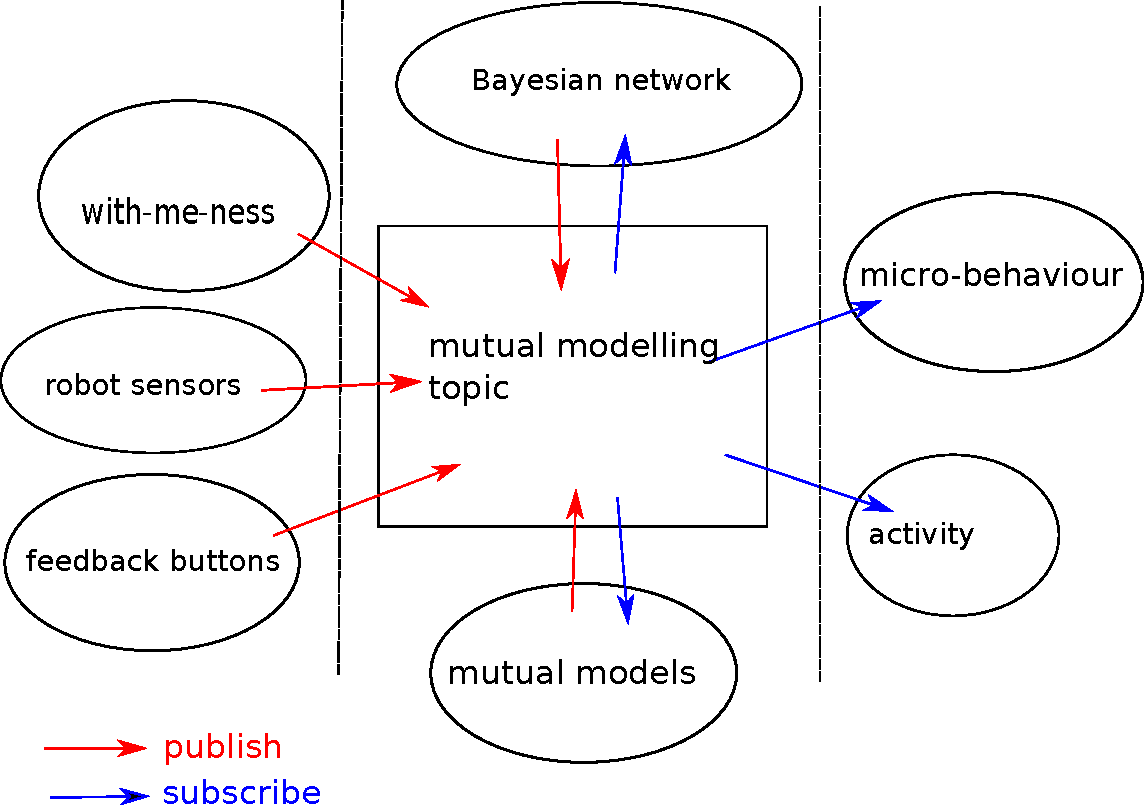
\includegraphics[width=0.8\columnwidth]{ros}
    \end{figure}
\end{frame}

%%%%%%%%%%%%%%%%%%%%%%%%%%%%%%%%%%%%%%%%%%%%%%%%%%%%%%%%%%%%%%%%%%%%%%%%%%%%%%%%
\section{Evaluation}

\begin{frame}{hypothesis}
\begin{itemize}
	\item \textit{Decisions made using additive information from second level of mutual modelling improve the quality of the CoWriter interaction.}
\end{itemize}
\end{frame}

\begin{frame}{Quality of the interaction ?}
\begin{enumerate}
	\item Quantity of demos
	\item Time spent to write demos
	\item Progress of child/robot
	\item With-me-ness
	\item Feedback buttons 
\end{enumerate}
\end{frame}

\begin{frame}{Experimental studies}
\begin{itemize}
	\item Long-term studies
	\item Children with real deficits
	\item Professional facilitators
\end{itemize}
\end{frame}

%%%%%%%%%%%%%%%%%%%%%%%%%%%%%%%%%%%%%%%%%%%%%%%%%%%%%%%%%%%%%%%%%%%%%%%%%%%%%%%%
\section{Conclusion \& planning}

\begin{frame}{Remind}
\begin{enumerate}
\item \textcolor{blue}{Question}: Does a second level of modelling\\enable higher quality interactions?
\item \textcolor{blue}{Hypothesis}: Yes.
\item \textcolor{blue}{Tools}: CoWriter activity + MM-cognitive architecture
\item \textcolor{blue}{Evaluation}: Long-term studies with children
\end{enumerate}
\end{frame}

\begin{frame}{Step by step approach}
\begin{itemize}
\item New variable (or group of variables)
\item New experiment to test the impact
\end{itemize}
\end{frame}

\begin{frame}
	\begin{figure}
        \centering
        \includegraphics[width=1.\columnwidth]{robots}
    \end{figure}
\end{frame}

\end{document}






